\problemWithTimeMem{Border Phony}{1 second}{1024MB}

scutsky和byyq是一对好朋友,他们经常一起学习各种有趣的算法。今天他们学习的内容是字符串的border的知识(若一个串T既是S的前缀,也是S的后缀,则认为串T是串S的border,\textbf{本题不考虑T=S的情况}。今天,scutsky想问byyq如何求得一个
字符串的最长border。byyq是一个codeforces还没有红名的newbie,所以他认为他需要去使用Binary Search
去解决这个问题,他构造的算法如下:

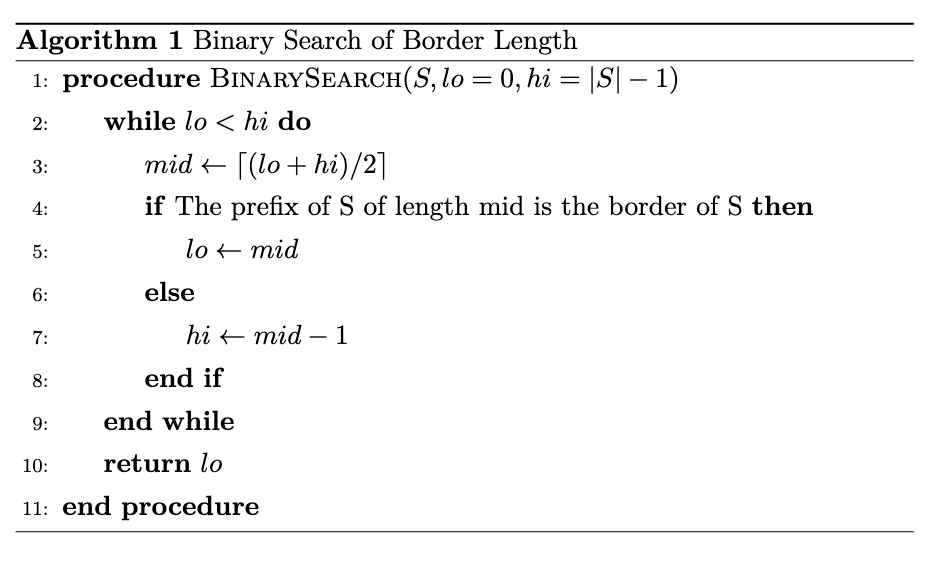
\includegraphics[width=.9\linewidth]{image4.png}

scutsky知道这个做法或许有点问题,但是他非常宠byyq,不想让他知道他的算法是错误的。而现在,他要给byyq出练习题了。
他已经决定了要构造一个长度为$n$的\textbf{由小写字母组成}的字符串,而最长border的长度为$m(0 \leqslant m < n)$,他希望byyq能用他的Binary Search算法去成功找到这个字符串的最长border,但是他并不知道应该构造一个什么样子的字符串,请你帮助scutsky完成这个出题任务。若不存在这样的字符串,请你输出"-1"表示无解。(不包含双引号)

\mysec{Input}

第一行包含一个整数 $T$($1 \leqslant T \leqslant 10^4$  ),接下来是$T$个测试样例。

对于每个测试样例,输入一行两个整数$n$,$m$($1\leqslant n \leqslant 3 \times 10^5 , 0 \leqslant m < n$)。

保证所有测试样例$\sum n\leqslant 3\times 10^5$。

\mysec{Output}

对于每个测试样例,输入一行一个字符串表示结果。

\ACMIO{Sample 1}{%
2

4 0

4 1
}{%
byyq

ajka
}
